\documentclass{beamer}
\usepackage[utf8]{inputenc}

\usetheme{Madrid}
\usecolortheme{default}
\usepackage{amsmath,amssymb,amsfonts,amsthm}
\usepackage{mathtools}
\usepackage{txfonts}
\usepackage{tkz-euclide}
\usepackage{listings}
\usepackage{adjustbox}
\usepackage{array}
\usepackage{gensymb}
\usepackage{tabularx}
\usepackage{gvv}
\usepackage{lmodern}
\usepackage{circuitikz}
\usepackage{tikz}
\lstset{literate={·}{{$\cdot$}}1 {λ}{{$\lambda$}}1 {→}{{$\to$}}1}
\usepackage{multicol}
\usepackage{graphicx}

\setbeamertemplate{page number in head/foot}[totalframenumber]

\usepackage{tcolorbox}
\tcbuselibrary{minted,breakable,xparse,skins}



\definecolor{bg}{gray}{0.95}
\DeclareTCBListing{mintedbox}{O{}m!O{}}{%
  breakable=true,
  listing engine=minted,
  listing only,
  minted language=#2,
  minted style=default,
  minted options={%
    linenos,
    gobble=0,
    breaklines=true,
    breakafter=,,
    fontsize=\small,
    numbersep=8pt,
    #1},
  boxsep=0pt,
  left skip=0pt,
  right skip=0pt,
  left=25pt,
  right=0pt,
  top=3pt,
  bottom=3pt,
  arc=5pt,
  leftrule=0pt,
  rightrule=0pt,
  bottomrule=2pt,
  toprule=2pt,
  colback=bg,
  colframe=orange!70,
  enhanced,
  overlay={%
    \begin{tcbclipinterior}
    \fill[orange!20!white] (frame.south west) rectangle ([xshift=20pt]frame.north west);
    \end{tcbclipinterior}},
  #3,
}
\lstset{
    language=C,
    basicstyle=\ttfamily\small,
    keywordstyle=\color{blue},
    stringstyle=\color{orange},
    commentstyle=\color{green!60!black},
    numbers=left,
    numberstyle=\tiny\color{gray},
    breaklines=true,
    showstringspaces=false,
}
%------------------------------------------------------------
%This block of code defines the information to appear in the
%Title page
\title %optional
{12.40}
\date{September 12,2025}
%\subtitle{A short story}

\author % (optional)
{Harsha-EE25BTECH11026}



\begin{document}


\frame{\titlepage}


\begin{frame}{Question}
If a rectangle is deformed into a parallelogram of equal area by simple shear deformation (with shear strain $\gamma$) parallel to the abscissa, the displacement matrix is \underline{\hspace{2cm}}.
\begin{enumerate}
\begin{multicols}{2}
    \item $\myvec{1&&\gamma\\0&&1}$
    \item $\myvec{1&&0\\\gamma&&1}$
    \item $\myvec{1&&0\\0&&1}$
    \item $\myvec{0&&\gamma\\1&&0}$
\end{multicols}
\end{enumerate}
\end{frame}

\begin{frame}{Theoretical Solution}
Due to the shear deformation, let $x',y'$ be the new coordinates. As the deformation is along the direction of abscissa,
\begin{align}
    \therefore y'=y \label{eq:1}
\end{align}
Let the displacement due to the shear deformation be $\Delta h$.
\begin{align}
    \gamma=\frac{\Delta h}{y}
\end{align}
\begin{align}
    \therefore \Delta h=\gamma y
\end{align}
\begin{align}
    \implies x'=x+\Delta h=x+\gamma y \label{eq:2}
\end{align}
From ~\eqref{eq:1} and ~\eqref{eq:2},
\begin{align}
    \therefore \myvec{x'\\y'}=\myvec{x+\gamma y \\ y}=\myvec{1&&\gamma\\0&&1}\myvec{x\\y}
\end{align}
\end{frame}


\begin{frame}[fragile]
    \frametitle{C Code -Finding displacement matrix}

    \begin{lstlisting}[language=C]
#include<stdio.h>

void displacement_matrix(double *matrix, double gamma){
	matrix[0]=1;
	matrix[1]=gamma;
	matrix[2]=0;
	matrix[3]=1;
}
    \end{lstlisting}
\end{frame}



\begin{frame}[fragile]
    \frametitle{Python+C code}

    \begin{lstlisting}[language=Python]
import ctypes
import sympy as sp
import numpy as np
import matplotlib.pyplot as plt

lib=ctypes.CDLL("./lib_dis_matrix.so")

lib.displacement_matrix.argtypes=(np.ctypeslib.ndpointer(dtype=np.float64, ndim=1, flags="C_CONTIGUOUS"),ctypes.c_double)

def shear_matrix(gamma: float) -> np.ndarray:
    mat = np.zeros(4, dtype=np.float64)  # flattened 2x2
    lib.displacement_matrix(mat, gamma)
    return mat.reshape((2, 2))

    \end{lstlisting}
\end{frame}

\begin{frame}[fragile]
    \frametitle{Python+C code}

    \begin{lstlisting}[language=Python]
# Example usage
gamma = 0.5
A= shear_matrix(gamma)
B=sp.Matrix(A)
print("Displacement matrix:\n")
sp.pprint(B)

# Define rectangle corners (counter-clockwise)
rect = np.array([[0, 0],
                 [2, 0],
                 [2, 1],
                 [0, 1],
                 [0, 0]])  # closed loop

# Apply shear transformation
deformed = rect @ B.T
    \end{lstlisting}
\end{frame}

\begin{frame}[fragile]
    \frametitle{Python+C code}

    \begin{lstlisting}[language=Python]
# Plot
plt.figure(figsize=(8, 8))
plt.plot(rect[:, 0], rect[:, 1], 'b-', label='Original Rectangle')
plt.plot(deformed[:, 0], deformed[:, 1], 'r--', label='Sheared Parallelogram')
plt.fill(rect[:, 0], rect[:, 1], 'b', alpha=0.2)
plt.fill(deformed[:, 0], deformed[:, 1], 'r', alpha=0.2)
plt.axhline(0, color='k', linewidth=0.5)
plt.axvline(0, color='k', linewidth=0.5)
plt.gca().set_aspect('equal', adjustable='box')
plt.legend(loc="upper right")
plt.title(f"Simple Shear Deformation (gamma = {gamma})")
plt.savefig("/home/user/Matrix Theory: workspace/Matgeo_assignments/12.456/figs/Figure_1.png")
plt.show()
    \end{lstlisting}
\end{frame}

\begin{frame}[fragile]
    \frametitle{Python code}
    \begin{lstlisting}[language=Python]
import sympy as sp
import numpy as np
import matplotlib.pyplot as plt

# Example
gamma = 0.5 
A=sp.Matrix([[1,gamma],[0,1]])
B=np.matrix([[1,gamma],[0,1]])
print("Displacement Matrix:\n")
sp.pprint(A)


# Define rectangle corners (counter-clockwise)
rect = np.array([[0, 0],
                 [2, 0],
                 [2, 1],
                 [0, 1],
                 [0, 0]])  # closed loop

    \end{lstlisting}   
\end{frame}

\begin{frame}[fragile]
    \frametitle{Python code}
    \begin{lstlisting}[language=Python]
# Apply shear transformation
deformed = rect @ B.T
# Plot
plt.figure(figsize=(8, 8))
plt.plot(rect[:, 0], rect[:, 1], 'b-', label='Original Rectangle')
plt.plot(deformed[:, 0], deformed[:, 1], 'r--', label='Sheared Parallelogram')
plt.fill(rect[:, 0], rect[:, 1], 'b', alpha=0.2)
plt.fill(deformed[:, 0], deformed[:, 1], 'r', alpha=0.2)
plt.axhline(0, color='k', linewidth=0.5)
plt.axvline(0, color='k', linewidth=0.5)
plt.gca().set_aspect('equal', adjustable='box')
plt.legend(loc="upper right")
plt.title(f"Simple Shear Deformation (gamma = {gamma})")
plt.savefig("/home/user/Matrix Theory: workspace/Matgeo_assignments/12.456/figs/Figure_1.png")
plt.show()
    \end{lstlisting}   
\end{frame}

\begin{frame}{Plot}
    \begin{figure}[H]
    \centering
    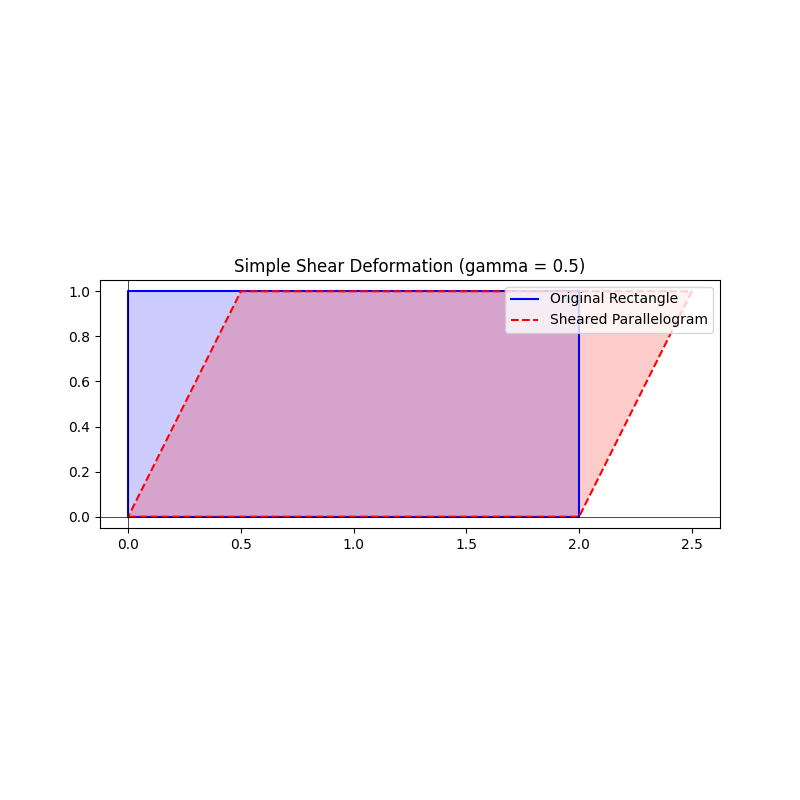
\includegraphics[width=0.6\columnwidth]{figs/Figure_1.png}
    \label{fig:1}
\end{figure}
\end{frame}

\end{document}